\documentclass[../../main.tex]{subfiles}
\begin{document}
\chapter{Facial Expressions}
\label{ch:facial_expressions}

Facial expressions are a crucial element of communication in both spoken and sign languages. In sign languages, they serve a dual purpose: conveying the emotional state of the signer and encoding grammatical information such as questions, negation, and emphasis. While spoken languages rely on tone and intonation for these functions, sign languages depend heavily on non-manual signals, particularly facial expressions, to fully convey the meaning of an utterance. Therefore, creating accurate and expressive facial animations in signing avatars is essential for producing realistic and comprehensible sign language content.

However, synthesizing facial expressions for signing avatars presents significant challenges due to the complexity and subtlety of these expressions. Unlike manual signs, which involve distinct hand and arm movements, facial expressions require the coordinated movement of various facial muscles, each contributing to the overall expression. Different facial features, such as eyebrows, eyes, and mouth, often move independently yet in harmony to produce coherent expressions. Moreover, the same facial expression can convey different meanings depending on the context, adding another layer of complexity to the task.

This chapter tackles these challenges by introducing a method for synthesizing facial expressions using the AZee framework for French Sign Language (LSF). To achieve this, specific production rules for facial expressions were integrated into AZee. By employing action units (AUs) as the foundational elements of these expressions, we can generate blendshapes that precisely represent the required facial movements. These blendshapes are subsequently integrated into a facial rigging system, allowing for the dynamic and realistic animation of signing avatars.

Previous chapters focused on the synthesis of manual features in sign language. In contrast, this chapter centers on the synthesis of facial expressions using the AZee framework, emphasizing their critical role in both emotional communication and the conveyance of grammatical information in sign languages. The precise synthesis of these expressions is therefore essential for enhancing the realism and effectiveness of signing avatars.

The chapter is structured as follows: Section~\ref{ch:facial_expressions:related_work} reviews related work in facial expression synthesis, examining previous approaches, the challenges encountered, and recent advancements. Section~\ref{ch:facial_expressions:related_work:facial_expressions_in_sign_language_synthesis} focuses on the synthesis of facial expressions in sign language avatars, discussing their importance for sign language comprehension and the challenges in capturing their nuances. Section~\ref{ch:facial_expressions:related_work:face_rigging} explores different face rigging techniques, including blendshape-based rigging, skeleton-based rigging, and hybrid methods, and compares their advantages and disadvantages. Finally, Section~\ref{ch:facial_expressions:related_work:emotion_recognition} delves into emotion recognition systems and their role in generating facial expressions that align with the emotional tone of the signed message.

\section{Related Work}
\label{ch:facial_expressions:related_work}

This section reviews the previous work in facial expression synthesis, focusing on the challenges and advancements in capturing the nuances of facial movements. It also discusses the importance of facial expressions in sign language synthesis and the techniques used to model these expressions effectively.

\subsubsection{Facial Expressions Synthesis}
\label{ch:facial_expressions:related_work:facial_expressions_synthesis}

Most of the facial expressions research is motivated by synthesis from voice signals. These methods are generally categorized into lip-sync techniques~\cite{yousaidthat, talkingface, lipmovements, lipsyncexpert}, which align mouth movements with audio, and full-face expression synthesis~\cite{eskimez, greenwood18, controllable_facial_synth}. Some approaches model speaking style with 3D animation parameters~\cite{cudeiro}, create generalized latent audio expressions combined with a person-specific 3D model~\cite{FLAME}, and produce expressive facial outputs conditioned on style, although some are unsuitable for tasks requiring full-face movement~\cite{imitating}. A related work, MakeItTalk~\cite{Yang:2020:MakeItTalk}, introduces a two-stage deep learning model that predicts facial landmark displacements based on audio input and a speaker identifier, followed by an image-to-image translation method to generate the final facial expression. Another study, EAMM~\cite{eamm}, focuses on transferring local emotional deformations to an audio-driven talking face, using deep learning to map audio to keypoints and their dynamics, resulting in emotion-related facial motions.

Synthesis of facial expressions in sign language is a much-less explored area. SGNify~\cite{Forte_2023_CVPR} can do a 3D reconstruction of a signer's face using in FLAME~\cite{FLAME} space from a monocular video. The Paula avatar uses rotational pivots and pre-defined movements, offering more natural and expressive facial animations~\cite{johnson-2022-improved}. More recent work~\cite{azevedo2024empowering} uses sentiment and semantic information to generate realistic facial expressions, achieving state-of-the-art results and outperforming existing approaches. However, these methods are limited in their ability to capture the full range of facial expressions in sign language, particularly the grammatical and emotional nuances that are essential for effective communication. However, these methods are limited in their ability to meaningully relate facial expressions to the signed message.

\subsection{Emotion Recognition}
\label{ch:facial_expressions:related_work:emotion_recognition}

Emotion recognition systems typically use machine learning algorithms to analyze facial features and identify the underlying emotional state. These systems can be trained on large datasets of facial images, which are annotated with emotional labels, to learn the relationships between facial movements and emotions. The most common approach to define emotions is the Ekman's Facial Action Coding System (FACS)~\cite{ekman1978facial}, which categorizes facial expressions into a set of action units (AUs) (figure~\ref{fig:action_units})  that correspond to specific muscle movements. Recent works by~\cite{luo2022learning} have shown that deep learning models can infer the set of active action units on a face image, which can be used to predict the underlying emotion. EMOCA~\cite{danvevcek2022emoca} is another work which reconstructs 3D faces from single images, accurately capturing emotional expressions by introducing an emotion-consistency loss, significantly improving the quality of reconstructed expressions over previous methods.

\begin{figure}
    \centering
    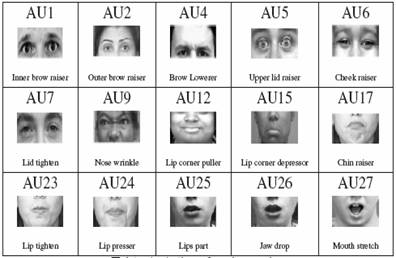
\includegraphics[width=0.8\textwidth]{chapters/facial_expressions/images/action_units.jpg}
    \caption{Facial Action Coding System (FACS) action units}
    \label{fig:action_units}
\end{figure}

Emotion recognition can be helpful in understanding as well as modeling facial expressions in sign language synthesis. By analyzing the emotional content of a signed message, we can generate facial expressions that align with the emotional tone of the message, enhancing the realism and expressiveness of the signing avatar.

\subsection{Face Rigging}
\label{ch:facial_expressions:related_work:face_rigging}

Face rigging is the process of creating a digital framework that allows for the animation of facial expressions. There are several approaches to face rigging, each with its advantages and disadvantages. The most common approaches include blendshape-based rigging and skeleton-based rigging.

\subsubsection{Blendshape-Based Rigging}
\label{ch:facial_expressions:related_work:face_rigging:blendshape_based_rigging}

Blendshape-based rigging involves creating a set of predefined facial shapes (blendshapes) that represent various expressions. These blendshapes can be blended together in different proportions to create a wide range of facial expressions. This method is widely used in the animation industry due to its simplicity and flexibility. It allows animators to create complex expressions by adjusting the influence of each blendshape on the final animation. However, the downside of this approach is that it requires a large number of blendshapes to capture all possible expressions, which can be time-consuming to create and manage.

Blendshapes are particularly effective for capturing specific facial movements, such as eyebrow raises, lip curls, cheek puffs, etc. By creating a library of blendshapes that correspond to different facial actions, animators can easily combine these shapes to create expressive and realistic facial animations (figure~\ref{fig:blendshapes}).

\begin{figure}
    \centering
    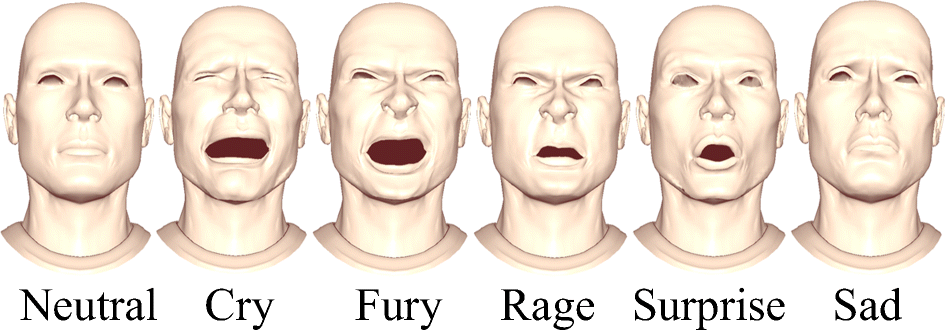
\includegraphics[width=0.8\textwidth]{chapters/facial_expressions/images/blendshapes.png}
    \caption{Blendshapes for facial expressions}
    \label{fig:blendshapes}
\end{figure}

\subsubsection{Skeleton-Based Rigging}
\label{ch:facial_expressions:related_work:face_rigging:skeleton_based_rigging}

Skeleton-based rigging, also known as joint-based rigging, uses a hierarchical system of bones and joints to control facial movements. This approach is more commonly used for animating body movements but can also be applied to facial animation. The advantage of skeleton-based rigging is that it provides a more ways to control since the control space of joints can be 3D (figure~\ref{fig:skeleton_based_rigging}). Example, jaw movements(up, down, left, right, front or back), eye movements, etc. However, it can be less intuitive to work with compared to blendshapes, especially for subtle expressions that require precise control over individual facial muscles.

\begin{figure}
    \centering
    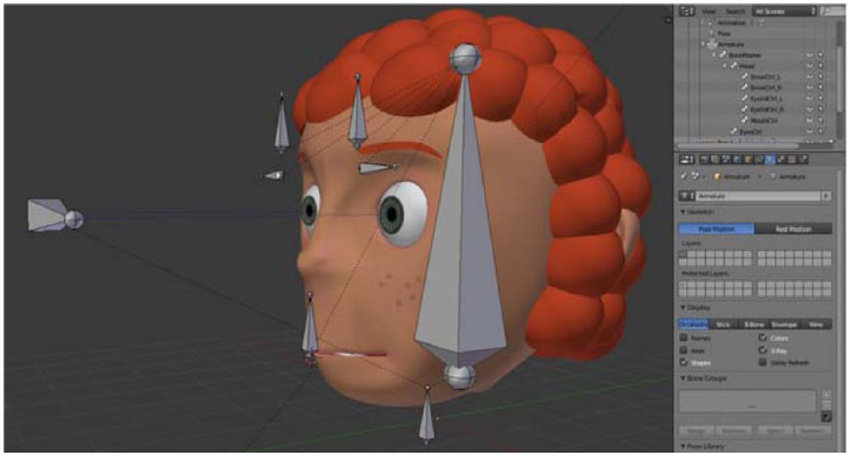
\includegraphics[width=0.8\textwidth]{chapters/facial_expressions/images/skeleton_based_rigging.png}
    \caption{Skeleton-based rigging for facial expressions}
    \label{fig:skeleton_based_rigging}
\end{figure}

\subsubsection{Hybrid Rigging}
\label{ch:facial_expressions:related_work:face_rigging:hybrid_rigging}

Hybrid rigging approaches combine elements of both blendshape-based and skeleton-based rigging to offer greater flexibility and control. By leveraging the strengths of both techniques, hybrid rigging can overcome the limitations of each individual approach. For example, blendshapes can be used for fine-tuned expressions, while skeletons provide control over broader movements like jaw or head rotations. 

\subsection{Capturing Facial Expressions}
\label{ch:facial_expressions:related_work:face_rigging:capture}

Keyframing remains a foundational technique in facial animation, where animators manually set key poses and interpolate between them to create fluid motion. While keyframing is effective in controlled environments, it may struggle to capture the natural variability and complexity required in sign language synthesis, where subtle changes in expression can convey different meanings.

\begin{figure}
    \centering
    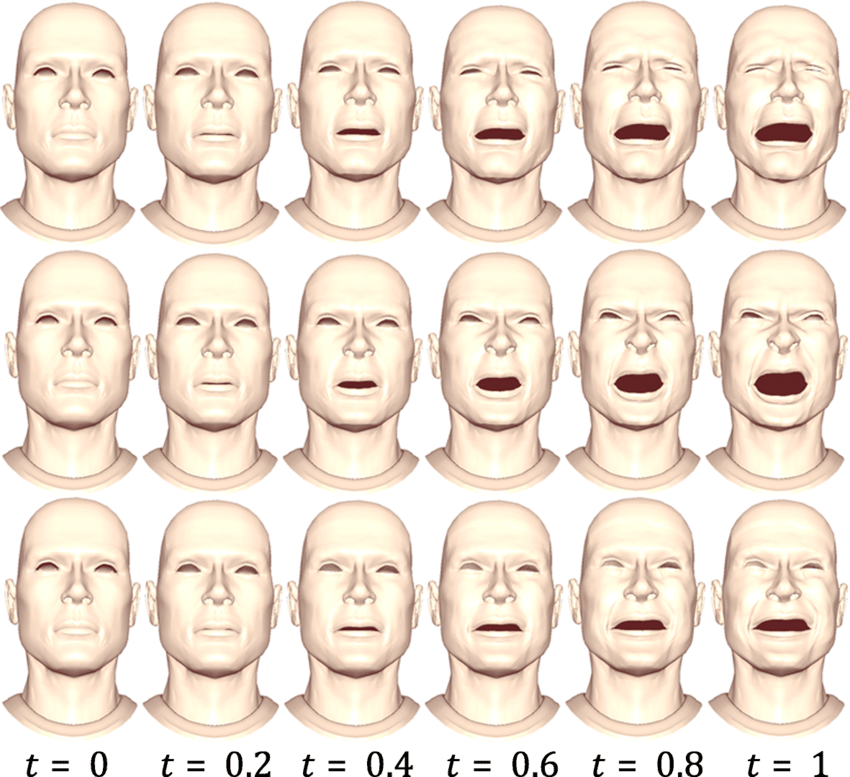
\includegraphics[width=0.8\textwidth]{chapters/facial_expressions/images/keyframing.png}
    \caption{Keyframing process, showing how key poses are set and interpolated to create a continuous animation.}
    \label{fig:keyframing}
\end{figure}

Performance-based approaches, such as motion capture, involve capturing real human facial movements and using this data to drive digital avatars. This method provides a high level of realism, capturing the natural dynamics and nuances of facial expressions. Apple's ARKit and FaceCap are examples of performance-based facial animation tools that use motion capture technology to animate digital characters (figure~\ref{fig:motion_capture}).

\begin{figure}
    \centering
    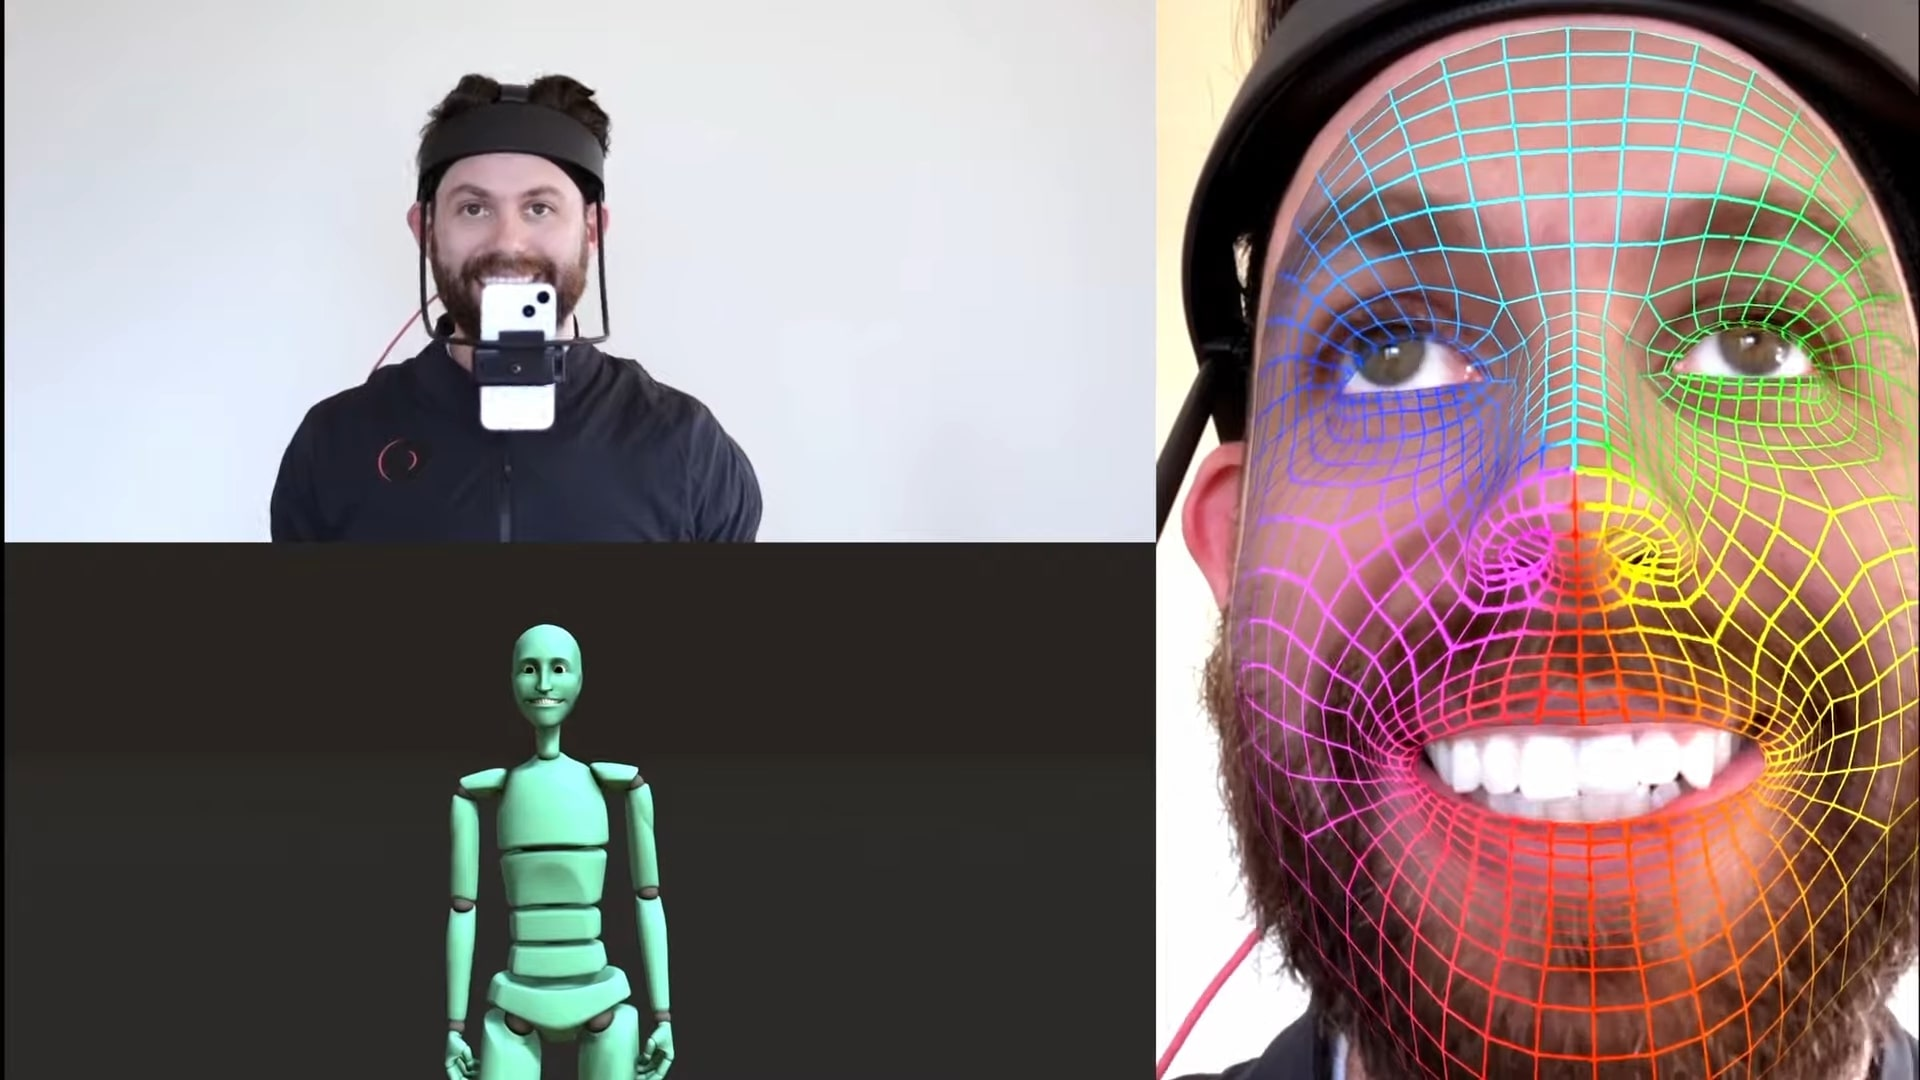
\includegraphics[width=0.8\textwidth]{chapters/facial_expressions/images/motion_capture.jpg}
    \caption{Performance-based facial animation using Apple's ARKit}
    \label{fig:motion_capture}
\end{figure}

\section{Action Unit Analysis}
\label{ch:facial_expressions:action_unit_analysis}

Our method for facial expression synthesis is based on the creation of blendshapes from action units (AUs), which are the fundamental building blocks of facial expressions as defined by the Facial Action Coding System (FACS). This section outlines the steps involved in our method, from the analysis of action units to the creation of blendshapes and the generation of motion curves.

The first step in our method is the analysis of action units (AUs). AUs represent the activation of specific facial muscles and are the basic components of facial expressions. Each AU corresponds to a particular movement, such as raising the eyebrows or pursing the lips, and can be combined with other AUs to create complex expressions.

To analyze AUs, we used a combination of manual observation and automatic detection tools. We also used mediapipe and the AU detector by~\cite{luo2022learning}, to identify AUs in still images (figure~\ref{fig:face_detect}). While these tools provided a useful starting point, they often required manual adjustments to ensure accuracy, particularly for subtle or complex expressions.

\begin{figure}
    \centering
    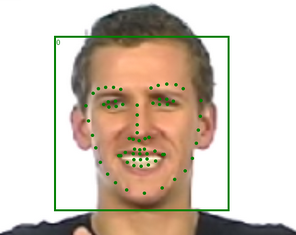
\includegraphics[width=0.8\textwidth]{chapters/facial_expressions/images/face_detect.png}
    \caption{Facial action unit detection using mediapipe and the AU detector by~\cite{luo2022learning} for \emph{big-threatening}}
    \label{fig:face_detect}
\end{figure}

For these manual adjustments, we used a linguists input by adjusting the movements of individual facial features(figure~\ref{fig:face_adjust}).

\begin{figure}
    \centering
    \includegraphics[width=0.8\textwidth]{chapters/facial_expressions/images/face_adjust.png}
    \caption{Manual adjustment of facial expressions to ensure accuracy.}
    \label{fig:face_adjust}
\end{figure}

The synthesized facial expressions were taken from our reference corpus (the 40 brèves corpus)~\cite{challant2024extending}~\cite{challant2022first}, breaking down each expression into its constituent AUs. This approach allowed us to ensure that our blendshapes accurately reflected the intended expressions, capturing both the emotional and grammatical nuances required for sign language synthesis.

\section{Blendshape Creation}
\label{ch:facial_expressions:blendshape_creation}

Once the AUs were identified, we used FACSHuman~\cite{gilbert2021facshuman} blendshapes as reference to create shapekeys in blender that correspond to each AU~\ref{fig:facshuman_blendshapes}. Shape keys~\ref{fig:shape_keys} are essentially different versions of a 3D model, each representing a specific change in vertices. By blending and interpolating these keys together, we can create a wide range of mesh shapes.

Since the FACSHuman blendshape work on any MakeHuman template mesh, this technique of synthesis is avatar independant. However, since the original model doesn't cover all the blendshapes(for all the face meshes), some blendshapes were created manually. The complete process involved iterating between manual adjustments and automated tools to ensure that the blendshapes accurately captured the intended expressions. The creation of blendshapes also involved ensuring that they could be seamlessly combined to create complex expressions. For example, the blendshape for AU4 (Brow Lowerer) was designed to work in conjunction with AU6 (Cheek Raiser) and AU12 (Lip Corner Puller) to create expressions of anger or determination. This required careful coordination of the vertex movements across different blendshapes to avoid unnatural deformations or artifacts in the final animation.

\begin{figure}
    \centering
    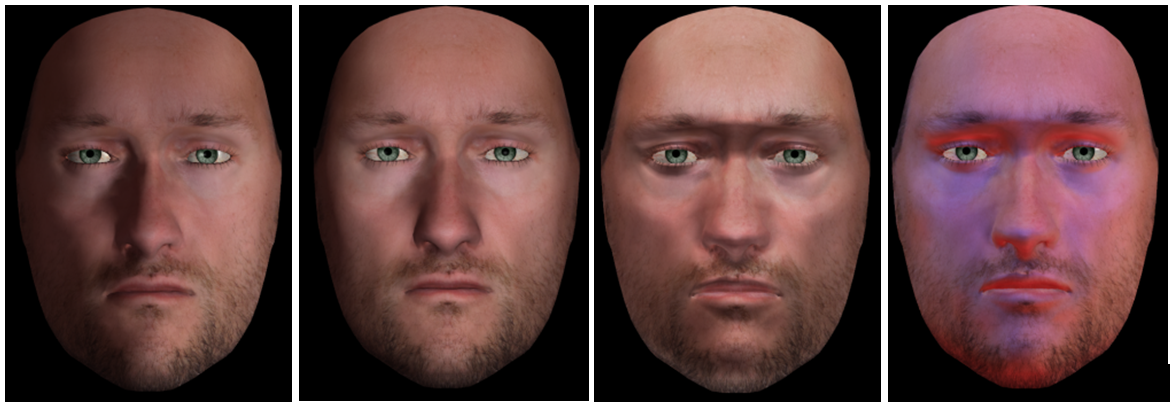
\includegraphics[width=0.8\textwidth]{chapters/facial_expressions/images/facshuman_blendshapes.png}
    \caption{FACSHuman blendshapes used as reference for creating shapekeys in blender.}
    \label{fig:facshuman_blendshapes}
\end{figure}

\begin{figure}
    \centering
    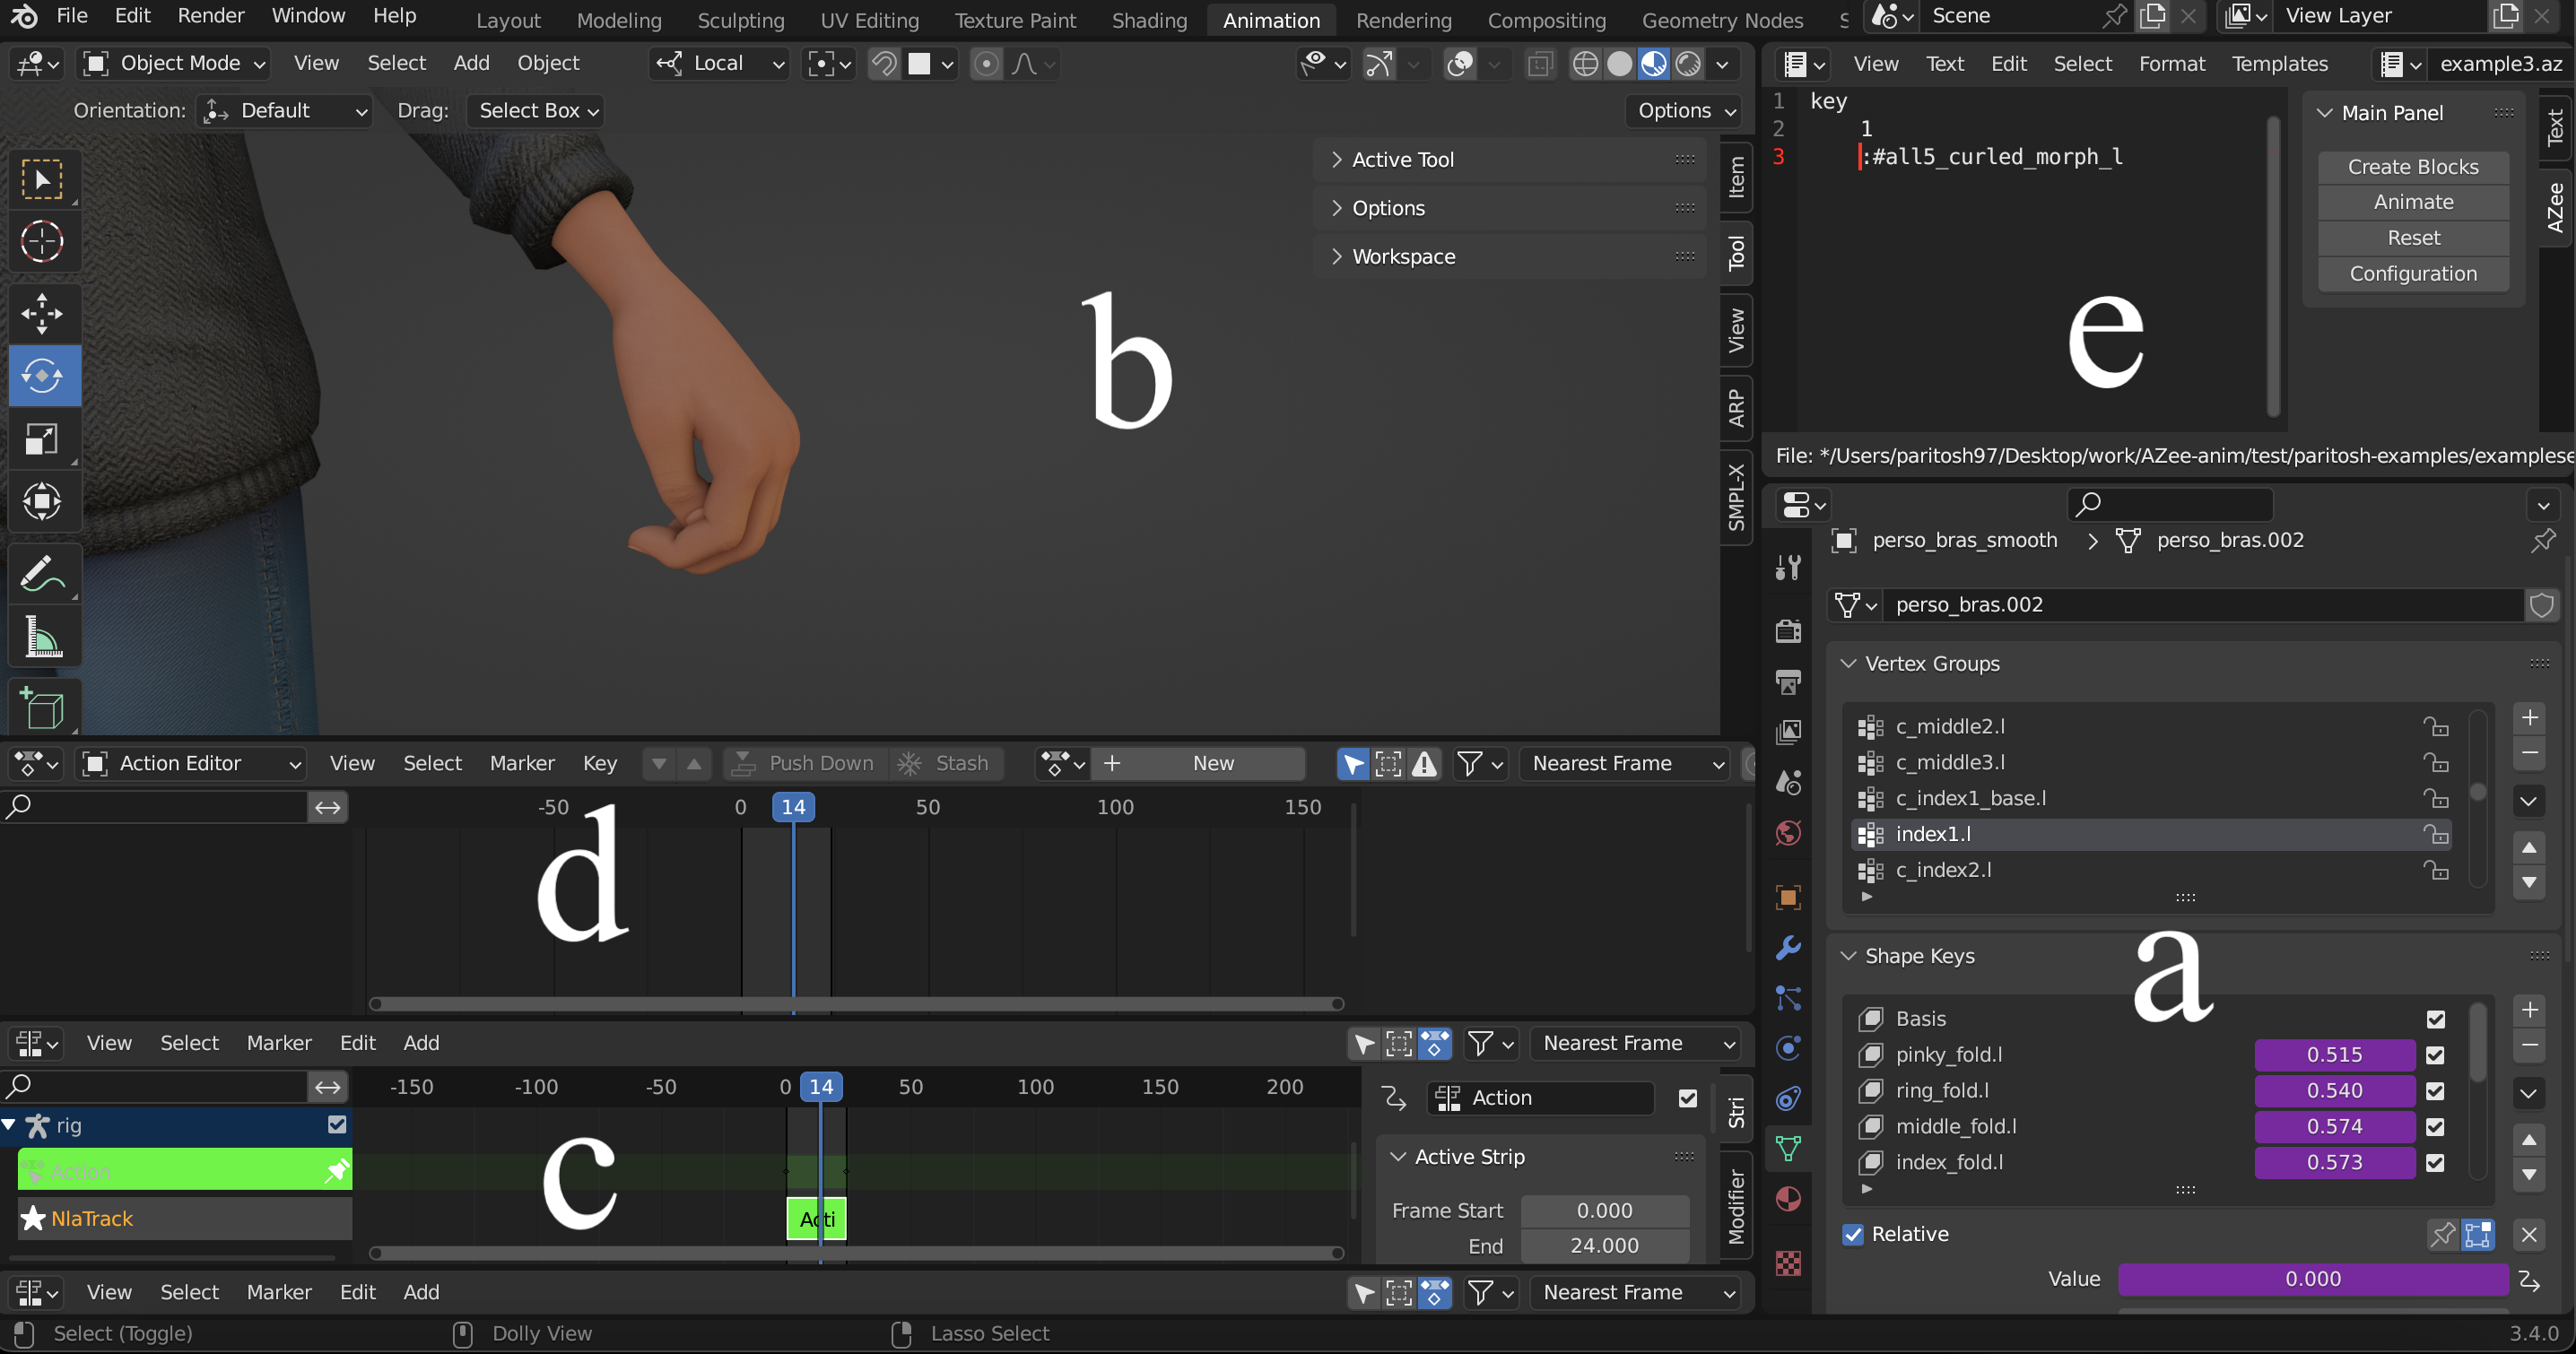
\includegraphics[width=0.8\textwidth]{chapters/facial_expressions/images/shape_keys.png}
    \caption{Blender interface. (a) Shape Key properties (b) 3D Viewport (c) Non-linear Editor (d) Action Editor (e) AZee editor}
    \label{fig:shape_keys}
\end{figure}

Lastly, we extended the low-level AZee language morph set with 94 blendshapes corresponding to most of the action units in the FACS system (figure~\ref{tab:added_units}) along with some additional ones. A few action units were not added~\ref{tab:not_added} since they were controlled by other skeletal constraints. Some morphs are also alternative blendshapes for the same action unit~\ref{tab:alternative_blendshapes} but with a different effect on the face.

\begin{table}[h]
    \centering
    \scriptsize
    \begin{tabular}{|c|l|c|l|}
        \hline
        \textbf{AU Code} & \textbf{Description}                     & \textbf{AU Code} & \textbf{Description}                      \\ \hline
        AU1              & Inner Brow Raise                        & AU1\_L            & Inner Brow Raise (Left)                   \\ \hline
        AU1\_R           & Inner Brow Raise (Right)                & AU2              & Outer Brow Raise                          \\ \hline
        AU2\_L           & Outer Brow Raise (Left)                 & AU2\_R            & Outer Brow Raise (Right)                  \\ \hline
        AU4              & Brow Lowerer                            & AU5              & Upper Lid Raise                           \\ \hline
        AU5\_L           & Upper Lid Raise (Left)                  & AU5\_R            & Upper Lid Raise (Right)                   \\ \hline
        AU6              & Cheek Raise                             & AU6\_L            & Cheek Raise (Left)                        \\ \hline
        AU6\_R           & Cheek Raise (Right)                     & AU7              & Lids Tight                                \\ \hline
        AU7\_L           & Lids Tight (Left)                       & AU7\_R            & Lids Tight (Right)                        \\ \hline
        AU8              & Lips Toward Each Other                  & AU9              & Nose Wrinkle                              \\ \hline
        AU9\_L           & Nose Wrinkle (Left)                     & AU9\_R            & Nose Wrinkle (Right)                      \\ \hline
        AU10             & Upper Lip Raiser                        & AU10\_L           & Upper Lip Raiser (Left)                   \\ \hline
        AU10\_R          & Upper Lip Raiser (Right)                & AU11             & Nasolabial Furrow Deepener                \\ \hline
        AU11\_L          & Nasolabial Furrow Deepener (Left)       & AU11\_R           & Nasolabial Furrow Deepener (Right)        \\ \hline
        AU12             & Lip Corner Puller                       & AU12\_L           & Lip Corner Puller (Left)                  \\ \hline
        AU12\_R          & Lip Corner Puller (Right)               & AU13             & Sharp Lip Puller                          \\ \hline
        AU13\_L          & Sharp Lip Puller (Left)                 & AU13\_R           & Sharp Lip Puller (Right)                  \\ \hline
        AU14             & Dimpler                                 & AU14\_L           & Dimpler (Left)                            \\ \hline
        AU14\_R          & Dimpler (Right)                         & AU15             & Lip Corner Depressor                      \\ \hline
        AU15\_L          & Lip Corner Depressor (Left)             & AU15\_R           & Lip Corner Depressor (Right)              \\ \hline
        AU16             & Lower Lip Depress                       & AU17             & Chin Raiser                               \\ \hline
        AU18             & Lip Pucker                              & AU19             & Tongue Show                               \\ \hline
        AU20             & Lip Stretch                             & AU20\_L           & Lip Stretch (Left)                        \\ \hline
        AU20\_R          & Lip Stretch (Right)                     & AU21             & Neck Tightener                            \\ \hline
        AU22\_25\_up\_down & Lip Funneler (Both Lips) & AU23             & Lip Tightener                             \\ \hline
        AU24             & Lip Presser                             & AU25             & Lips Part                                 \\ \hline
        AU25\_L          & Lips Part (Left)                        & AU25\_R           & Lips Part (Right)                         \\ \hline
        AU26             & Jaw Drop                                & AU27             & Mouth Stretch                             \\ \hline
        AU28             & Lips Suck                               & AU29             & Jaw Thrust                                \\ \hline
        AU30\_L          & Jaw Sideways (Left)                     & AU30\_R           & Jaw Sideways (Right)                      \\ \hline
        AU31             & Jaw Clencher                            & AU32             & Bite                                      \\ \hline
        AU33             & Blow                                    & AU34             & Puff                                      \\ \hline
        AU35             & Cheek Suck                              & AU36             & Tongue Bulge                              \\ \hline
        AU37             & Lip Wipe                                & AU38             & Nostril Dilate                            \\ \hline
        AU39             & Nostril Compress                        & AU43             & Eye Closure                               \\ \hline
        AU43\_L          & Eye Close (Left)                        & AU43\_R           & Eye Close (Right)                         \\ \hline
    \end{tabular}
    \caption{Added blend shapes} 
    \label{tab:added_units} 
\end{table}

\begin{table}
    \centering
    \scriptsize
    \begin{tabular}{|c|l|c|l|}
        \hline
        \textbf{AU Code} & \textbf{Description}                     & \textbf{AU Code} & \textbf{Description}                      \\ \hline
        AU40             & Sniff                                   & AU41             & Lid Droop                                 \\ \hline
        AU42             & Slit                                    & AU44             & Squint                                    \\ \hline
        AU45             & Blink                                   & AU46             & Wink                                      \\ \hline
        AU51             & Head Turn Left (IK controlled)          & AU52             & Head Turn Right (IK controlled)           \\ \hline
        AU53             & Head Up (IK controlled)                 & AU54             & Head Down (IK controlled)                 \\ \hline
        AU55             & Head Tilt Left (IK controlled)          & AU56             & Head Tilt Right (IK controlled)           \\ \hline
        AU57             & Head Forward (IK controlled)            & AU58             & Head Back (IK controlled)                 \\ \hline
        AU61             & Eyes Turn Left (lookat constraint)      & AU62             & Eyes Turn Right (lookat constraint)       \\ \hline
        AU63             & Eyes Up (lookat constraint)             & AU64             & Eyes Down (lookat constraint)             \\ \hline
    \end{tabular}
    \caption{Action units skipped} 
    \label{tab:not_added} 
\end{table}


\vspace{1cm}

\begin{table}
    \centering
    \scriptsize
    \begin{tabular}{|c|l|c|l|}
        \hline
        \textbf{AU Code} & \textbf{Description}                     & \textbf{AU Code} & \textbf{Description}                      \\ \hline
        AU1\_a            & Inner Brow Raise (Alternative)          & AU2\_a            & Outer Brow Raise (Alternative)           \\ \hline
        AU4\_a            & Brow Lowerer (Alternative A)            & AU4\_b            & Brow Lowerer (Alternative B)             \\ \hline
        AU6\_a            & Cheek Raise (Alternative A)             & AU6\_b            & Cheek Raise (Alternative B)              \\ \hline
        AU9\_a            & Nose Wrinkle (Alternative A)            & AU12\_a           & Lip Corner Puller (Alternative A)        \\ \hline
        AU12\_b           & Lip Corner Puller (Alternative B)       & AU17\_a           & Chin Raiser (Alternative A)              \\ \hline
        AU18\_a           & Lip Pucker (Alternative)                & AU25\_a           & Lips Part (Alternative A)                \\ \hline
        AU22\_25\_upper  & Lip Funneler (Upper Lip)     & AU22\_25\_down   & Lip Funneler (Bottom Lip)  \\ \hline
        AU26\_lip\_down   & Jaw Drop Bottom Lip Down (Alternative)  & AU26\_tongue\_down & Jaw Drop Tongue Down (Alternative)       \\ \hline
        AU26\_tongue\_out & Jaw Drop Tongue Out (Alternative)       & AU26\_a           & Jaw Drop (Alternative)                   \\ \hline
        AU28\_a           & Lips Suck (Upper Lip)                   & AU28\_bottom      & Lips Suck (Lower Lip)                    \\ \hline
        tongue\_back\_up  & Tongue Back Up                          & tongue\_out       & Tongue Out                               \\ \hline
        tongue\_up        & Tongue Up                               & tongue\_wide      & Tongue Wide                              \\ \hline
    \end{tabular}
    \caption{Alternative blend shapes} 
    \label{tab:alternative_blendshapes}
\end{table}



\subsection{Motion Curves for Blendshapes}
\label{ch:facial_expressions:motion_curves_for_blendshapes}

After creating the blendshapes, we generated motion curves (more discussed in~\ref{ch:intermediate_blocks}) to control how these shapes are animated over time. Motion curves define the changes in the blendshape's influence over the course of an animation, allowing for smooth transitions between different facial expressions.

We extended our intermediate block generation algorithm to include motion curves for facial morphs. This involved creating additional curves that specify the timing and intensity of facial movements based on the template. By controlling the acceleration and deceleration of these movements, we were able to create more naturalistic animations that reflect the dynamic nature of facial expressions.

For example, in the expression "big-threatening," the motion curves were designed to gradually increase the influence of the blendshapes corresponding to AU10 (Upper Lip Raiser) and AU25 (Lips Part) while simultaneously decreasing the influence of AU4 (Brow Lowerer) as the expression transitions from a neutral state to one of aggression (figure~\ref{fig:motion_curve_example}). This careful modulation of the blendshape influences over time resulted in an expression that not only looked realistic but also conveyed the intended emotional and grammatical cues effectively.

\begin{figure}
    \centering
    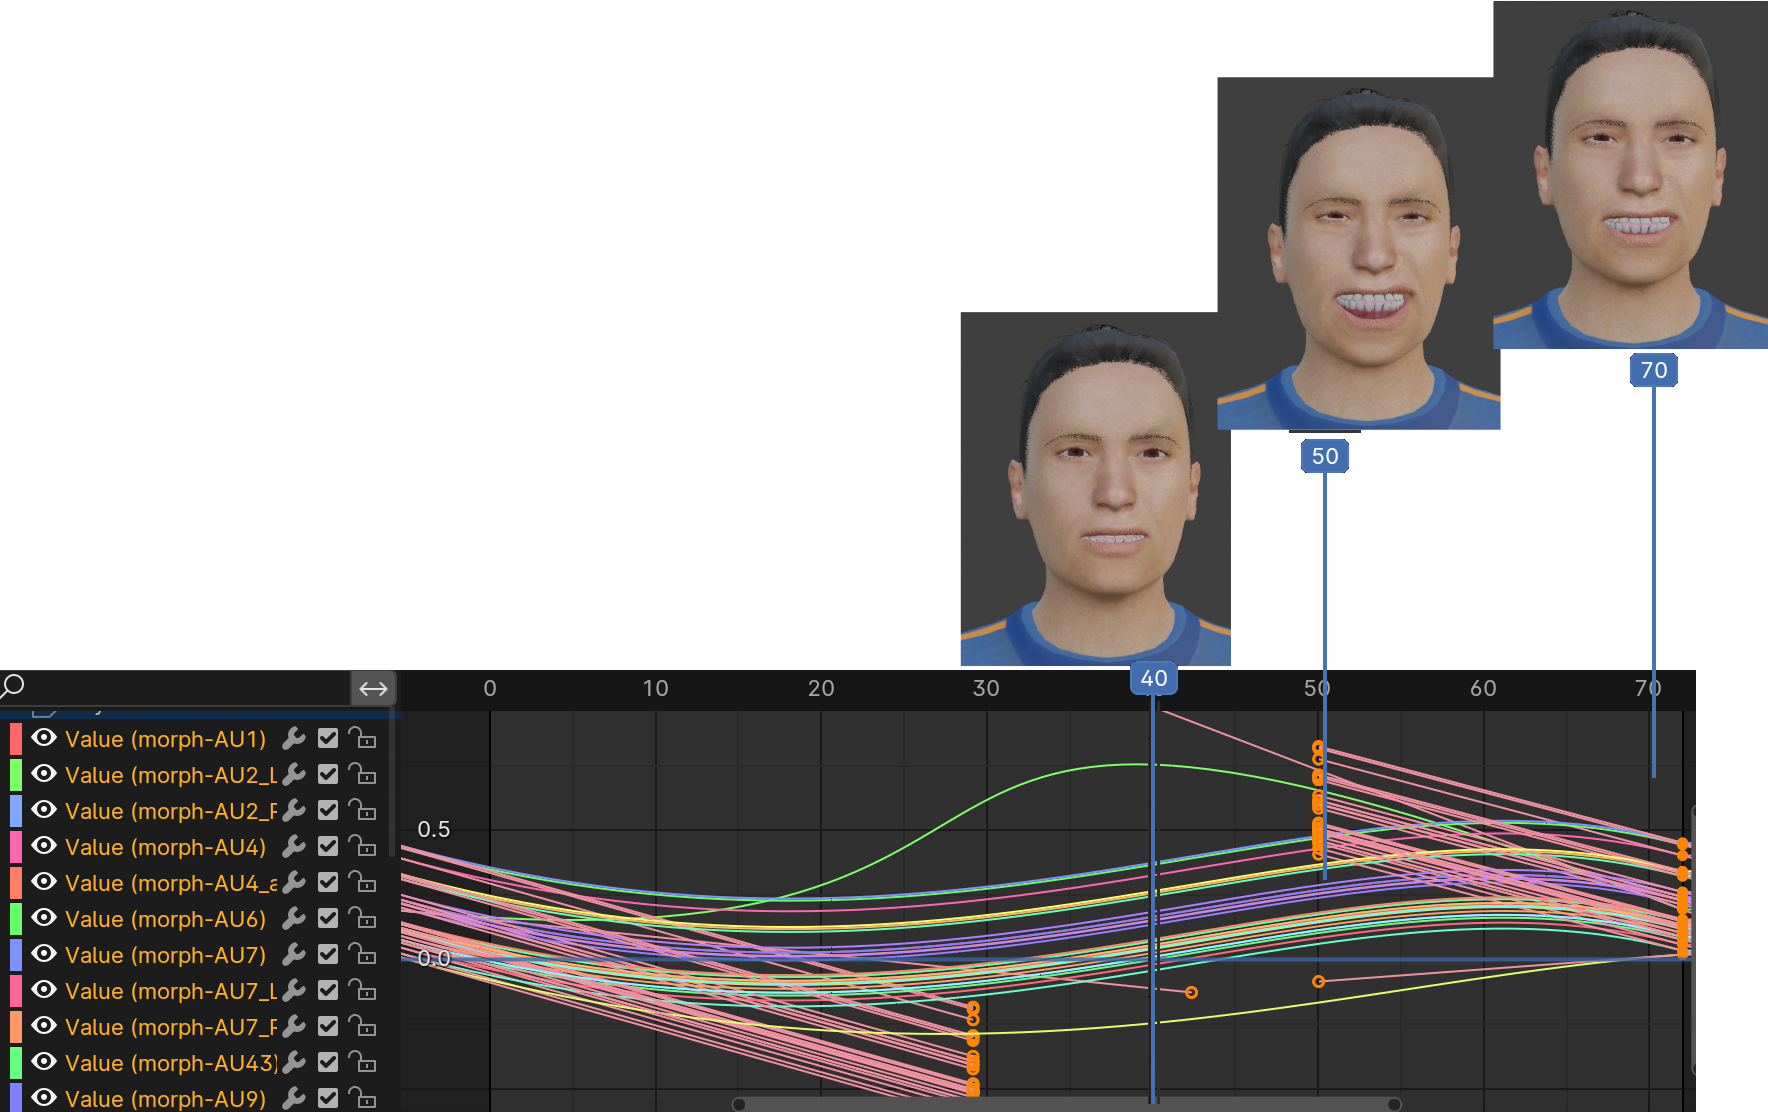
\includegraphics[width=0.8\textwidth]{chapters/facial_expressions/images/motion_curve_example.png}
    \caption{Motion curves controlling the blendshape influences for the expression "big-threatening."}
    \label{fig:motion_curve_example}
\end{figure}

\section{Results and Evaluation}
\label{ch:facial_expressions:results}

Synthesis of all the facial expressions from the 40 brèves corpus can be seen in table~\ref{tab:facial_expressions}. The expressions were created by combining the relevant blendshapes  to produce realistic and expressive facial animations.


\begin{table}
    \centering
    \begin{tabular}{|c|c|c|}
        \hline
        \textbf{Expression} & \textbf{Description} & \textbf{Blendshapes} \\
        \hline
        AZee & Facial Expression \\
        todo & todo \\
    \end{tabular}
    \caption{Facial expressions synthesized using the AZee framework.}
    \label{tab:facial_expressions}
\end{table}

\section{Evaluation}
\label{ch:facial_expressions:evaluation}

Table~\ref{tab:facial_expressions_evaluation} shows the subjective evaluation by a linguist of the facial expressions synthesized using the AZee framework. The expressions were assessed based on their accuracy, expressiveness, and effectiveness in conveying the intended emotional and grammatical cues.

\begin{table*}
    \centering
    \begin{tabular}{|l|p{8cm}|}
    \hline
    \textbf{Expression} & \textbf{Limitations} \\
    \hline
    \texttt{almost-reaching} & Mouth modeling unconvincing. \\
    \hline
    \texttt{continuously} & "Pffff" air and cheek puff difficult, neutral eyebrows. \\
    \hline
    \texttt{do-you-realise} & Thick eyebrow issue. \\
    \hline
    \texttt{it-is-a-shame} & Mouth expression not quite real. \\
    \hline
    \texttt{most-probably} & Less visible teeth preferred, thick eyebrow issue. \\
    \hline
    \texttt{much-almost-too-much} & Frowning eyebrows and lack of eye wrinkles not convincing. \\
    \hline
    \texttt{nothing-sticks-out} & Tucked lips difficult to model. \\
    \hline
   \texttt{something-sticks-out} & Interpreted as confusion, mouth modeling limitation. \\
    \hline
    \texttt{trouble-disturbance} & Frowning eyebrows difficult, mouth "rising" hard to model, result not convincing. \\
    \hline
    \texttt{uneasy-awkward} & Tongue tip out with slightly open mouth hard to model, unconvincing. \\
    \hline
    \texttt{with-chaos} & Single cheek blow/puff and alternating eye blinks hard without animation. \\
    \hline
    \texttt{with-no-precision} & Upper lip over lower and mouth near nose unmodellable. \\
    \hline
    \texttt{with-surprise} & Cannot lower lower eyelid fully, thick eyebrow issue. \\
    \hline
    \texttt{with-uncertainty} & Appears sadder than uncertain, thick eyebrow issue. \\
    \hline
    \texttt{with-worry} & Lack of wrinkles around nose/forehead. \\
    \hline
    \end{tabular}
    \caption{Limitations for each facial expression rule.}
    \label{tab:facial_expressions_evaluation}
\end{table*}

We observe that expressions that involved subtle mouth movements, such as "it-is-a-shame" or "something-sticks-out," were more challenging to model accurately, highlighting areas for further refinement.

Table~\ref{tab:facial_expressions_quantitative} shows the quantitative evaluation of the facial expressions using the Frechet Expression Distance (FED). We also fitted FLAME~\cite{FLAME} on the  ground truth facial expressions~\ref{fig:spectre} and compared them to the expressions synthesized using our method framework. The FED scores provide a measure of the similarity between the ground truth and synthesized expressions, with lower scores indicating a closer match.

\begin{figure}
    \centering
    \includegraphics[width=0.8\textwidth]{chapters/facial_expressions/images/sgnify.png}
    \caption{Facial expressions generated using FLAME by fitting SPECTRE}
    \label{fig:spectre}
\end{figure}

\begin{table}
    \centering
    \begin{tabular}{|c|c|}
        \hline
        \textbf{Expression} & \textbf{FED Score} \\
        \hline
        big-threatening & todo \\
        \hline
    \end{tabular}
    \caption{Quantitative evaluation of facial expressions synthesized}
    \label{tab:facial_expressions_quantitative}
\end{table}

The FED scores indicate that the synthesized expressions closely matched the ground truth expressions, demonstrating the effectiveness of our method in capturing the nuances of facial movements.

We also compare the synthesized utterance (with facial expressions) with the original utterance (without facial expressions) to evaluate the impact of facial expressions on sign language comprehension. For this we synthesize the following AZee description.

\begin{verbatim}    
    todo
\end{verbatim}

The following link shows the comparison between the two versions (and the SGNify version for inference) of the utterance:  \href{todo}. We observe that the added facial expressions todo...

\section{Conclusion}
\label{ch:facial_expressions:conclusion}

Facial expressions play a crucial role in sign language communication, conveying both emotional and grammatical information. In this chapter, we presented a method for synthesizing facial expressions using the AZee framework, focusing on the creation of blendshapes from action units (AUs) and the generation of motion curves to control these shapes over time. Our method involved analyzing AUs from the FACS system, creating blendshapes based on these AUs, and generating motion curves to animate the blendshapes. The synthesized facial expressions were evaluated subjectively by a linguist and quantitatively using the Frechet Expression Distance (FED) metric, demonstrating the effectiveness of our method in capturing the nuances of facial movements. The results show that the synthesized expressions closely matched the ground truth expressions, highlighting the potential of our method for enhancing the realism and expressiveness of signing avatars. Future work will focus on refining the blendshapes and motion curves to improve the accuracy and naturalness of the facial expressions, as well as exploring the integration of emotion recognition systems to generate facial expressions that align with the emotional tone of the signed message. By continuing to develop and refine our method, we aim to create more realistic and effective facial animations for sign language synthesis, enhancing the overall quality and accessibility of sign language content.


\end{document}